% Chapter 4

\chapter{Diseño}
% Write in your own chapter title
\label{Capitulo 4}
\lhead{Capítulo 4. \emph{Diseño}} % Write in your own chapter title to set the page header

%Al considerar los objetivos planteados en la introducción y los conflictos planteados en el capítulo anterior, surge la necesidad de desarrollar una alternativa que incorpore la sensibilidad al contexto a las aplicaciones web desarrolladas con continuations.
Al considerar los objetivos planteados en la introducción, que promueven la incorporación de la sensibilidad al contexto a las aplicaciones web desarrolladas con continuations, y los conflictos planteados en el capítulo anterior; surge la necesidad de diseñar una abstracción que busque una buena relación entre la sensibilidad al contexto y la privacidad del usuario.

La alternativa propuesta en esta tesis consiste en la creación de una librería que permita conocer el estado de los sensores del cliente desde el servidor, manteniendo la capacidad \emph{transaccional} de las aplicaciones web basadas en continuations, a la vez que se intenta mantener la \emph{privacidad del usuario} proporcionada por los navegadores web convencionales.

A continuación se detallan las decisiones de diseño tomadas comenzando desde el navegador web y culminando en el servidor. Primero se analizará la \emph{privacidad del usuario} en el cliente. Luego se prosigue con el \emph{mecanismo de suscripción/notificación en el cliente}, para posteriormente explicar el mismo \emph{mecanísmo visto desde el servidor}.

Por último se describe el proceso necesario para \emph{brindar soporte a un nuevo sensor}, y se presenta el \emph{modelo final}.


\section{Privacidad del usuario}

La privacidad del usuario de una aplicación web se encuentra determinada tanto por los navegadores web, como por la forma en que fue desarrollada esa aplicación.

La privacidad proporcionada por los navegadores web convencionales, consiste en aislar la ejecución de la aplicación web de una gran cantidad de información disponible en un dispositivo (como archivos, otros dispositivos conectados, sensores, etc).

Por otro lado, dado que la sensibilidad al contexto requiere información específica del usuario, es necesario acceder a cierta información protegida por la mayoría de los navegadores web (valores de los sensores que permitan reconocer el entorno del dispositivo, y a su vez parte del entorno del usuario).

Una forma de permitir el acceso a esta información desde las aplicaciones web se logra al proporcionar una API\footnote{Del inglés ``Application Programming Interface''.} que acceda a los valores de los sensores. Además, el navegador web, deberá proporcionar una interfaz para que el usuario pueda establecer a que información puede acceder la aplicación web.

Por ejemplo, el navegador web utilizado para la realización de esta tesis\footnote{Construido como consecuencia de la escasez de este tipo de navegadores web.}(basado en Phonegap) al presionar la tecla menú (en un dispositivo móvil) muestra una lista de sensores, desde donde se podrá seleccionar cuales serán compartidos mediante la API (Ver Figura \ref{PhoneGapBrowserLike}).

\begin{figure}[ht!]
\centering
\framebox[2.01in]{
\noindent
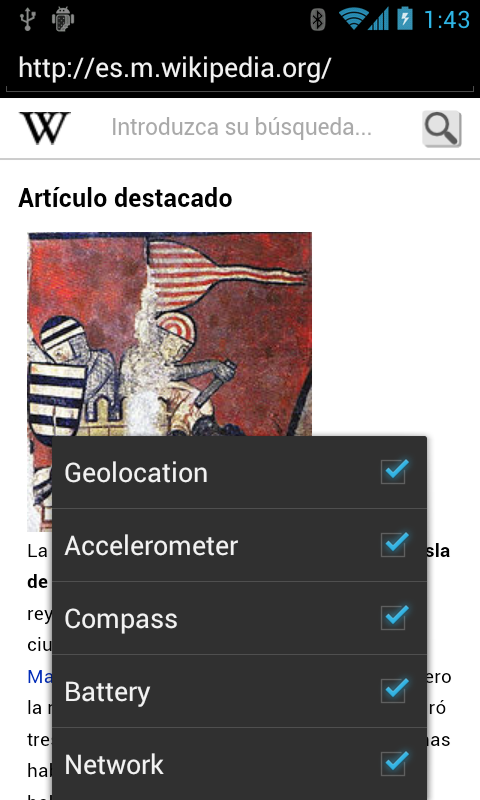
\includegraphics[scale=0.3]{Screenshot_2012-06-03-01-43-29}
}
\caption{Captura de pantalla del navegador web Phonegap}
\label{PhoneGapBrowserLike}
\end{figure}

Luego, dentro de las aplicaciones web, las interfaces (disponible desde Javascript) dependen de la velocidad con que se actualiza la información del sensor.

Aquellos sensores que recuperan información altamente cambiante (como el acelerómetro, el compás y la posición) proporcionan una interfaz para configurar un \emph{timer}\footnote{Tarea que se ejecuta de forma reiterativa dado cierto intervalo de tiempo.} mediante una función que requiere de 3 parámetros (ver Figura \ref{PhonegapAPI}, linea 4).

\begin{figure}[ht!]
\begin{Verbatim}
succes = function (listened) { };
fail = function (error) { };
options = { frequency: 1000 };
timerId = navigator.geolocation.watchPosition( sucess , fail , options );
\end{Verbatim}
\caption{Ejemplo de API en el lenguaje javascript para los sensores altamente cambiantes}
\label{PhonegapAPI}
\end{figure}

Los 2 primeros parmámetros son \emph{callbacks} (ver lineas 1 y 2) y el último un diccionario con \emph{opciones} de configuración (ver linea 3). El primer callback se ejecuta cuando se ha podido obtener la información de forma correcta, y el  otro en caso de que el sensor se haya encontrado con algún inconveniente.

Por otra parte, aquellos sensores que recuperan información menos dinámica (como la batería, la red a la que se encuentra conectado, etc.) suelen proveer una función para solicitar el valor actual.

Estas herramientas proporcionadas por el navegador web para que el usuario pueda seleccionar que parte de su contexto desea compartir son una parte de la solución al problema de la privacidad. La otra parte de la solución se encuentra en la forma que se encuentra desarrollada la aplicación web.

Si se tiene en cuenta la privacidad del usuario al momento de diseñar una aplicación web, existen ciertas decisiones de diseño que pueden ser tomadas.

Un aspecto importante de la privacidad del usuario, es reducir al mínimo la transferencia de información de los sensores hacia los servidores, comunicando solo aquella información que sirva para tomar una decisión en el servidor.

Este tipo de optimización, puede ser realizada al utilizar el patrón de diseño \emph{Publish/Subscriber} descripto por \emph{Birman et al.}\cite{Birman87}, que permite registrarse a un entorno de interés, en lugar de requerir que el cliente envíe el estado de sus sensores de forma continua.

De esta forma, el servidor deberá registrarse a un entorno determinado (mediante algún mecanismo de \emph{Server Push}) y el cliente realizará la notificación pertinente cuando el entorno sea compatible con el contexto del usuario.


\section{Mecanismo de suscripción a un entorno}

Para realizar una suscripción a un entorno, es necesario diseñar una estructura que detalle las características que permiten describirlo.

Hay entornos que dependen de la información de un solo sensor, mientras que existirán otros que dependen de una combinación de varios. Inclusive, sería deseable, que se puedan definir \emph{sub-entornos} que luego puedan ser reutilizados en diferentes entornos mas complejos.

Para obtener esta \emph{granularidad} en la definición del entorno, se utiliza el patrón de diseño \emph{Composite} descripto por \emph{Gamma et al.}\cite{Gamma95}, mediante las clases \emph{Condition}, \emph{SimpleCondition} y \emph{ComplexCondition} (ver Figura \ref{CompositeCondition}).

\begin{figure}[ht!]
\centering
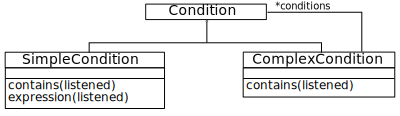
\includegraphics[scale=1]{ConditionComposite}
\caption{Implementación del patrón Composite mediante la clase Condition}
\label{CompositeCondition}
\end{figure}

La clase \emph{SimpleCondition} representa al estado deseado de un sensor en un momento determinado. Es la menor granularidad posible dentro de la definición del entorno, pudiendo evaluarse si el estado de un sensor cumple con su requisito mediante el método \emph{contains}.

Por otra parte, la clase \emph{ComplexCondition} permite la caracterización de entornos a partir de la utilización de varios sensores. Cuando se evalúa una condición compleja (utilizando el método \emph{contains}) se tiene en cuenta que todas las condiciones que la componen se cumplan. En caso de no cumplirse alguna de las condiciones, la condición compleja tampoco se cumplirá.

Por último, para homogeneizar las distintas interfaces (o API) con las que se puede acceder a la información de un sensor (mediante el patrón de diseño \emph{Adapter}\cite{Gamma95}), se crea la clase \emph{Listener} que abstrae a las \emph{SimpleCondition} de la API específica del Phonegap (ver Figura \ref{ListenerAbstraction}).

\begin{figure}[ht!]
\centering
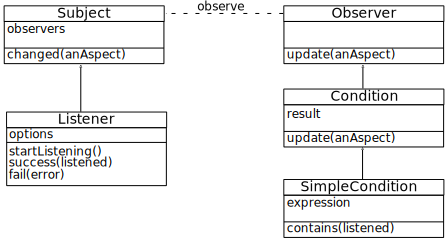
\includegraphics[scale=1]{ListenerAbstraction}
\caption{Abstracción de los sensores mediante la clase Listener}
\label{ListenerAbstraction}
\end{figure}

Dentro de una instancia de la clase \emph{Listener}, el método \emph{startListening} se encargará de inicializar un \emph{timer} (o, dependiendo del caso, de configurar el \emph{timer} perteneciente a la API de Phonegap) que será el encargado de leer el valor. En caso de éxito se llamará al método \emph{success} y en caso de error al método \emph{fail}.

Cada instancia de \emph{SimpleCondition} observará (mediante el patrón de diseño \emph{Observer} presentado por \emph{Gamma et al.}\cite{Gamma95}) a una instancia de la clase \emph{Listener}. De esta forma, cuando un \emph{Listener} conozca una nueva lectura de su sensor, las \emph{SimpleCondition} que lo observan podrán actuar al respecto.

Este proceso se encuentra detallado dentro del método \emph{success} de la clase \emph{Listener} en donde se notifica a cada \emph{SimpleCondition} que se encuentra observando, utilizando el método \emph{update}. Dentro de \emph{update}, cada \emph{SimpleCondition} evaluará si contiene (utilizando el método \emph{contains}) al valor informado por el sensor.

Una vez definidas las clases que permitirán la descripción y detección del entorno, es necesario detallar el mecanismo de notificación al servidor.


\section{Notificación al servidor de la ocurrencia de un entorno}

Teniendo en cuenta que el servidor se suscribió a un entorno detallado (descrípto por un conjunto de condiciones), cuando el cliente realice la notificación no requerirá el envío de información sobre el entorno.

El cliente solo informará cual es el \emph{callback de continuations} que el servidor debe ejecutar mediante una solicitud \emph{AJAX}, la cual ha sido administrada por el servidor al momento de registrarse al cliente. El cliente guarda dicha solicitud de forma \emph{serializada} en el atributo \emph{callback} de la clase \emph{Trigger}.

Luego, una instancia de la clase \emph{Trigger} se relaciona con una instancia de la clase \emph{Condition}, quedando asociado la descripción de un entorno determinado con una notificación al servidor (ver Figura \ref{TriggerNotification}).

\begin{figure}[ht!]
\centering
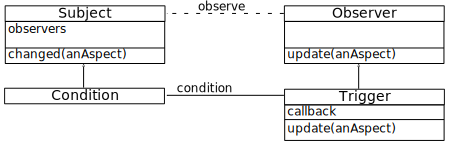
\includegraphics[scale=1]{TriggerNotification}
\caption{Implementación de la clase Trigger como parte escencial del patrón Public/Subscriber}
\label{TriggerNotification}
\end{figure}

Notar que la clase \emph{Condition} además de ser un \emph{observador} es un \emph{subjeto}, a partir de esto podrá ser observada por una instancia de la clase \emph{Trigger} o por una instancia de \emph{ComplexCondition}.

De esta forma, cuando la clase \emph{Listener} recupera un nuevo valor del sensor, se lo notifica a todas las \emph{SimpleCondition} que lo observan. Éstas, dependiendo del caso particular, notificarán a las \emph{ComplexCondition} (que podrán notificar a otras \emph{ComplexCondition}), hasta llegar a todos los \emph{Trigger} involucrados (ver Figura \ref{SequenceNotificationDiagram}).

\begin{figure}[ht!]
\centering
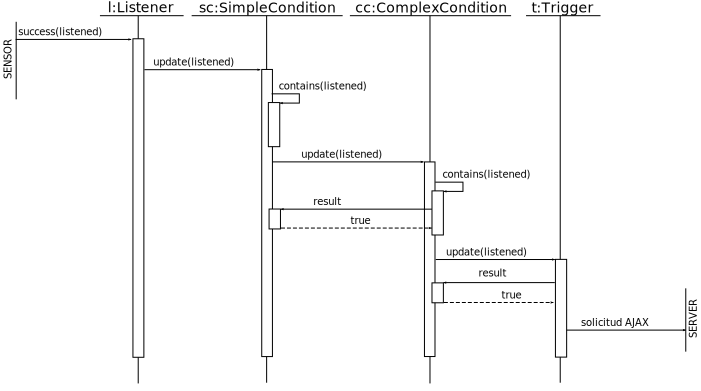
\includegraphics[scale=0.73]{SequenceNotificationDiagram}
\caption{Diagrama de secuencia UML del proceso de notificación}
\label{SequenceNotificationDiagram}
\end{figure}

Cada vez que un \emph{Trigger} es notificado de una actualización en su atributo \emph{condition}, verifica si la condición describe al entorno actual. En caso positivo, enviará la solicitud AJAX al servidor, informándole cual es el \emph{callback} que debe ejecutar.


\subsection{Optimización de la propagación}

Cada vez que el \emph{listener} notifica a las condiciones que lo observan, estas propagarán la notificación hasta llegar a los respectivos \emph{triggers} asociados (ver Figura \ref{SequenceNotificationFalseDiagram}).

\begin{figure}[ht!]
\centering
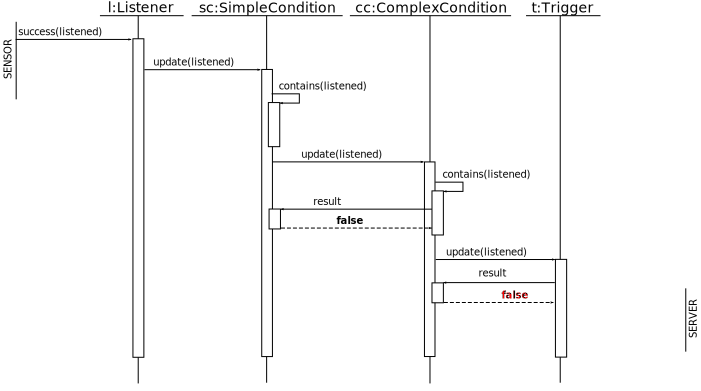
\includegraphics[scale=0.73]{SequenceNotificationFalseDiagram}
\caption{Diagrama de secuencia UML de la propagación hasta llegar al Trigger}
\label{SequenceNotificationFalseDiagram}
\end{figure}

El trigger es el que verifica si se debe notificar al servidor mediante la solicitud AJAX. Una forma de optmizar esto es frenar la propagación de la notificación en las condiciones previas, antes de que llegue al trigger, si es que la situación lo permite.

Para realizar esto se almacena el resultado de cada evaluación para cada condición. Esto permite verificar si la condición cambió de resultado con respecto a la evaluación anterior, permitiendo interrumpir la propagación en aquellos casos que lo requieran (ver Cuadro \ref{PropagationTable}).

\begin{table}[ht!]
\centering
\begin{tabular}{ | l | l l |}
\hline
anterior/actual & falso & verdadero \\
\hline
falso & para & continua \\
verdadero & continua & continua \\
\hline
\end{tabular}
\caption{Propagación de la notificación en las condiciones}
\label{PropagationTable}
\end{table}

Como se observa en la tabla cuando el resultado de la evaluación de una condición es \emph{falso}, y su resultado anterior fue \emph{falso} no es necesario notificar un cambio a los observadores de esta condición.


\section{Mecanismo de cancelación de una suscripción en el cliente}

Al considerar la interacción de un modelo con el contexto de sus usuarios, es posible contemplar que en algún momento el servidor deseará cancelar alguna de sus suscripciones.

Para poder realizar la cancelación es necesario que el servidor mantenga identificados todos los objetos enviados al cliente (triggers, condiciones simples y complejas). De esta forma puede especificarle al cliente cual de todos esos objetos quiere eliminar (o cancelar). Para lograrlo es necesario modificar la jerarquía de clases antes presentada, haciendo que la clase \emph{Condition} y la clase \emph{Trigger} extiendan a la clase \emph{ProxyObject} (ver Figura \ref{ProxyObjectHierarchy}).

\begin{figure}[ht!]
\centering
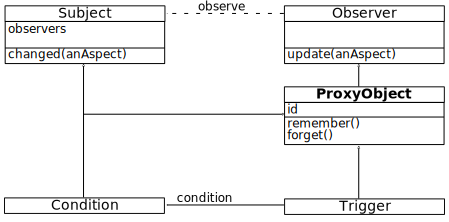
\includegraphics[scale=0.73]{ProxyObjectHierarchy}
\caption{Diagrama de clases UML con la clase ProxyObject}
\label{ProxyObjectHierarchy}
\end{figure}

Además la clase \emph{Contidion} continuará extendiendo a la clase \emph{Subject} para poder notificar a sus observadores en caso de ser necesario.

Por último es necesario subrayar que la clase \emph{ProxyObject} es la que permite reutilizar los \emph{sub-entornos} definidos utilizando instancias de la clase \emph{ComplexCondition}.


\section{Suscripción y desuscripción desde la perspectiva del servidor}

Teniendo en cuenta el esquema de notificaciones del cliente basados en el \emph{ProxyObject}, es necesario ampliar como el servidor construye la información para que luego pueda ser interpretada por el navegador web.

El proceso comienza cuando a una instancia de la clase \emph{Listener} (que reside en el servidor), asociada a un cliente en particular, se le envía el mensaje \emph{\#remember:} con una instancia de \emph{Trigger} como parámetro (ver Figura \ref{ServerSerializer}).

\begin{figure}[ht!]
\centering
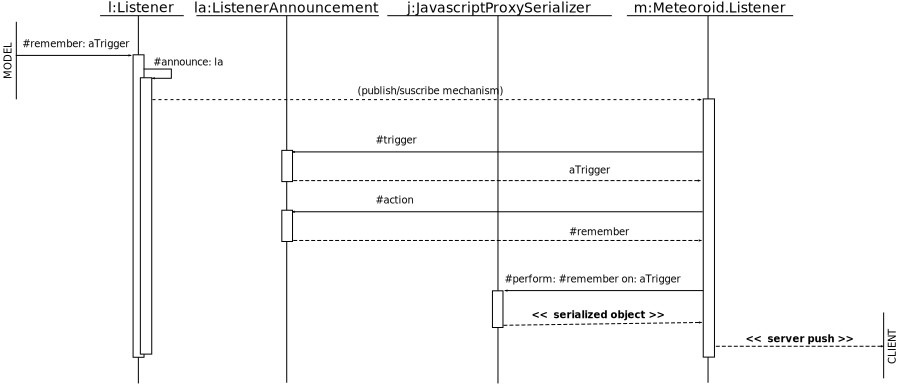
\includegraphics[scale=0.83,angle=90]{ServerSerializer}
\caption{Diagrama de secuencia UML de la serialización de objetos en el servidor}
\label{ServerSerializer}
\end{figure}

La instancia de la clase \emph{Listener} es observada por la clase \emph{Meteoroid.Listener}, que es un componente del framework \emph{Meteoroid}. Al utilizar el patrón de diseño \emph{Publish/Suscriber}, el componente de meteoroid es notificado cada vez que al Listener se le indica \emph{recordar} o \emph{olvidar} algún trigger.

Luego, al recibir una notificación la instancia de \emph{Meteoroid.Listener} le delega a una instancia de la clase \emph{JavascriptProxySerializer} para que recorra al objeto \emph{Trigger} con el fin de transformarlo en un código javascript adecuado para el navegador web.

El código javascript resultante describirá a las \emph{condiciones} que debe cumplir el entorno para ejecutar ese \emph{Trigger} y almacenará un \emph{callback de continuations} codificado como una solicitud de AJAX.

Por último, cuando el serializador devuelve el código javascript, el componente lo inyecta en el cliente (utilizando la técnica conocida como Server Push).


\section{Implementación de un sensor}

En las secciones anteriores se presentó el mecanismo de notificación de entornos en forma general. Este mecanismo le permite al servidor (basado en continuations) interactuar con un cliente dentro del dominio de la adaptabilidad al contexto. Para concluir con el entendimiento de lo explicado se prosigue con el desarrollo de un caso particular, como es el caso del \emph{sensor} de \emph{aceleración}.

Teniendo en cuenta que la aceleración proviene de un sensor altamente cambiante, el navegador web basado en \emph{Phonegap} provee en su API un método para configurar un \emph{timer}.

Para \emph{adaptar} esta API, se crea la clase \emph{AccelerationListener} (ver Figura \ref{AccelerationListenerClass}) que extiende a la clase \emph{Listener} e integra al sensor al mecanismo de notificaciones antes descripto.

\begin{figure}[ht!]
\begin{Verbatim}
AccelerationListener = Class.create(Listener, {
  initialize: function($super) {
    $super(1000);
  },
  sucess: function($super, listened) {
    _.listeners.acceleration.changed(listened);
    return true;
  },
  startListening: function() {
    this.timerId = navigator.accelerometer.watchAcceleration(
      this.sucess,
      this.fail,
      this.options
    );
  }
});

_.feel("acceleration", new AccelerationListener());
\end{Verbatim}
\caption{Código fuente de la clase AccelerationListener}
\label{AccelerationListenerClass}
\end{figure}

En el momento que este fragmento de código es interpretado por el navegador web, primero crea la clase \emph{AccelerationListener} y luego solicita al administrador de \emph{listeners} (clase \emph{ListenerManager}) para que agregue una instancia de la clase recién creada (linea 18). A partir de este momento una \emph{SimpleCondition} puede registrarse para escuchar una ``acceleration''.

En el proceso de creación de la instancia de la clase \emph{AccelerationListener}, por defecto se inicializa con una velocidad de refresco de \emph{1000 ms} que la clase \emph{Listener} se encargará de agregar al diccionario almacenado en el atributo \emph{options} (Ver linea 3 de la Figura \ref{AccelerationListenerClass}).

Luego, cuando se termine de cargar la página web, se le enviará un mensaje al método \emph{startListening} para que termine de configurar el \emph{timer} provisto por la interfaz de Phonegap (Ver linea 11 de la Figura \ref{AccelerationListenerClass}).

Cuando la aplicación web se encuentre corriendo en el cliente, cada vez que el \emph{timer} lo indique se llamará al método \emph{success}. Este último, se encarga de enviar el mensaje \emph{changed} a la instancia del listener para propagar la nueva lectura a todas las \emph{SimpleCondition} que lo estén observando (Ver linea 6 de la Figura \ref{AccelerationListenerClass}). A partir de esta propagación cada \emph{SimpleCondition} evaluará si contiene al valor propagado por el listener utilizando el atributo \emph{expression}.

Desde el punto de vista del desarrollador es necesario proporcionar una herramienta que simplifique la creación de condiciones. Para esto, en el servidor se implementa el patrón de diseño Builder explicado por \emph{Gamma et al.}\cite{Gamma95}.

Luego, para cada sensor se puede proporcionar un Builder que contemple los casos específicos de dicho sensor. Por ejemplo, para el caso del acelerómetro, se crea la clase \emph{OSCAccelerationBuilder} (ver Figura \ref{ServerBuilders}).

\begin{figure}[ht!]
\centering
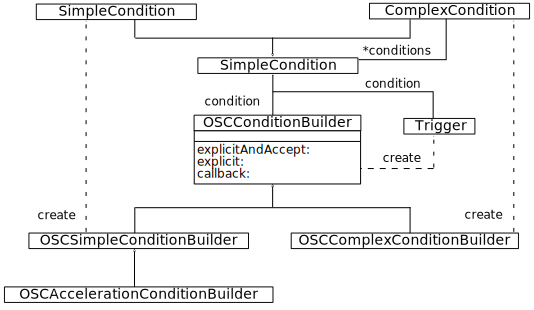
\includegraphics[scale=0.83]{ServerBuilders}
\caption{Diagrama de clases UML de la jerarquía de \emph{builders}}
\label{ServerBuilders}
\end{figure}

De esta forma, la clase \emph{OSCAccelerationBuilder} tiene la responsabilidad de construir instancias de la clase \emph{SimpleCondition} que serán atendidas por el listener que se encuentra del lado del cliente, registrado para atender condiciones de ``acceleration''.

Por último, como se observa en el diagrama de clases UML (Ver Figura \ref{ServerBuilders}) la librería cuenta con la clase \emph{OSCComplexConditionBuilder} que permite construir entornos complejos como consecuencia de agrupar un conjunto de condiciones.


\section{Visión global}

Con la misión de mantener, en la medida de lo posible, las características y propiedades de las aplicaciones web basadas en continuations, se diseña una extensión que permita la adaptación al contexto y mantienga la privacidad del usuario. Como se puede ver en el diagrama de clases \emph{UML}\footnote{Del inglés ``Unified Modeling Language''.} de la Figura \ref{UMLClassDiagram}, dicha extensión tiene dos partes, una se encuentra del lado del servidor y la otra del lado del cliente.

Para mantener dicha privacidad se plantea un esquema de notificaciones mediante el patrón de diseño \emph{Publish/Suscribe} que evita que el cliente deba enviar información detallada de los sensores al servidor. Para lograrlo, cada notificación del cliente solicitará al servidor que realice la ejecución de un \emph{callback de continuations} del framework \emph{Seaside}, de forma similar a la forma de procesar clicks en hipervinculos o botones.

\begin{figure}[ht!]
\centering
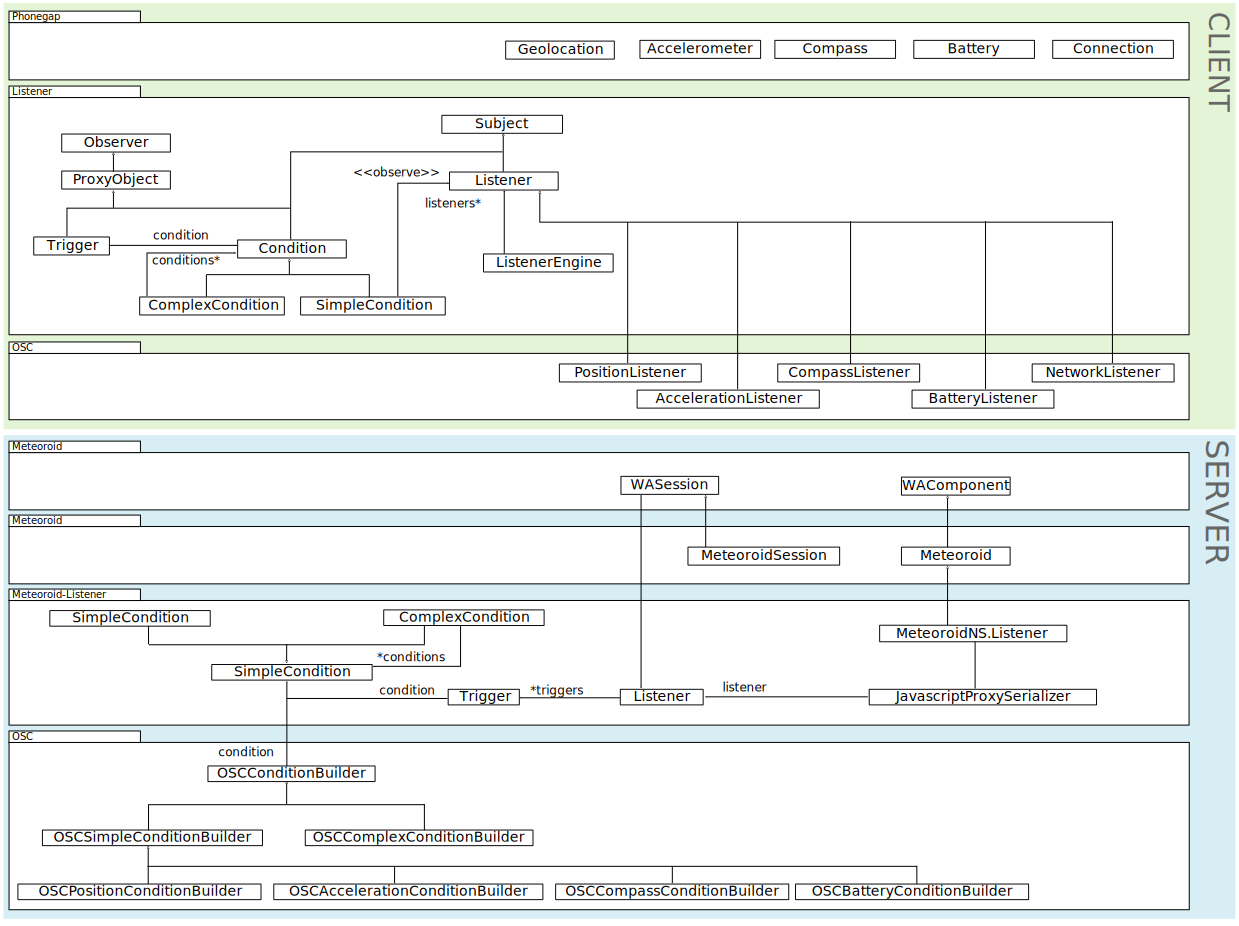
\includegraphics[scale=0.55,angle=90]{UMLClassDiagram}
\caption{Diagrama de clases UML de la extensión propuesta}
\label{UMLClassDiagram}
\end{figure}